\section{Sample System Ouput - State Data}
\begin{figure}[H]
	\centering
	\caption{qbar vs. Time}
		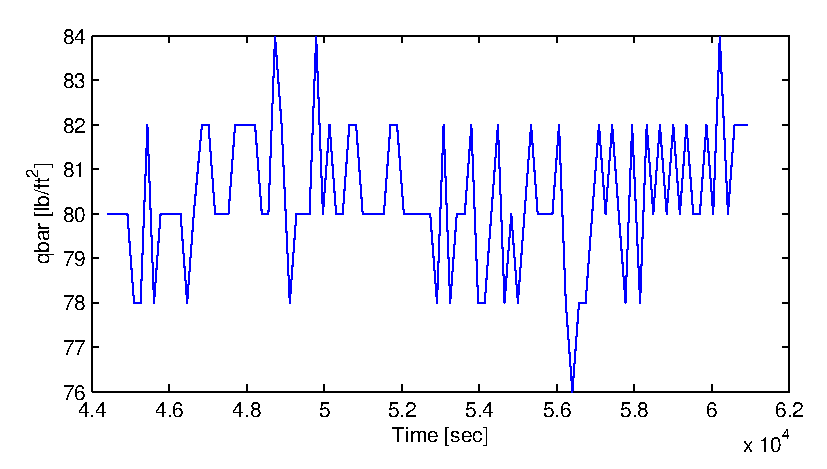
\includegraphics[width = 0.7\textwidth]{C:/Users/mufasa/Documents/Thesis/LaTex/figures/sampleOutput/State/qbar.eps}
\end{figure}
\begin{figure}[H]
	\centering
	\caption{rho vs. Time}
		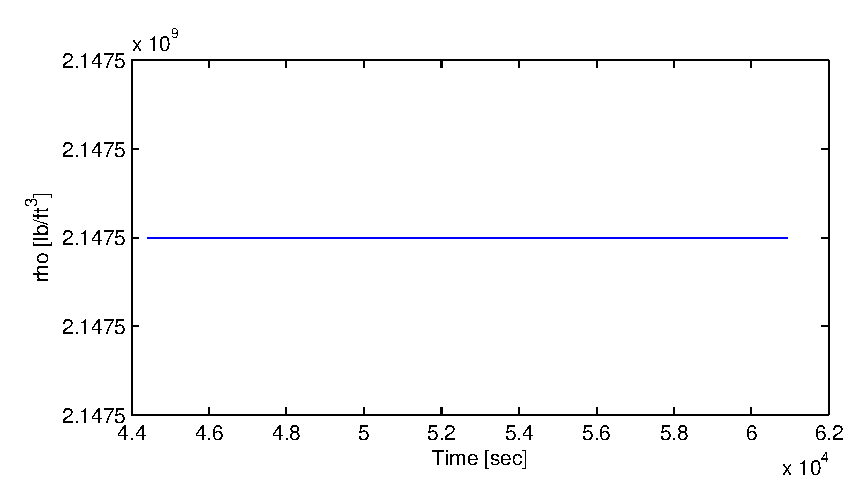
\includegraphics[width = 0.7\textwidth]{C:/Users/mufasa/Documents/Thesis/LaTex/figures/sampleOutput/State/rho.eps}
\end{figure}
\clearpage
\begin{figure}[H]
	\centering
	\caption{vinf vs. Time}
		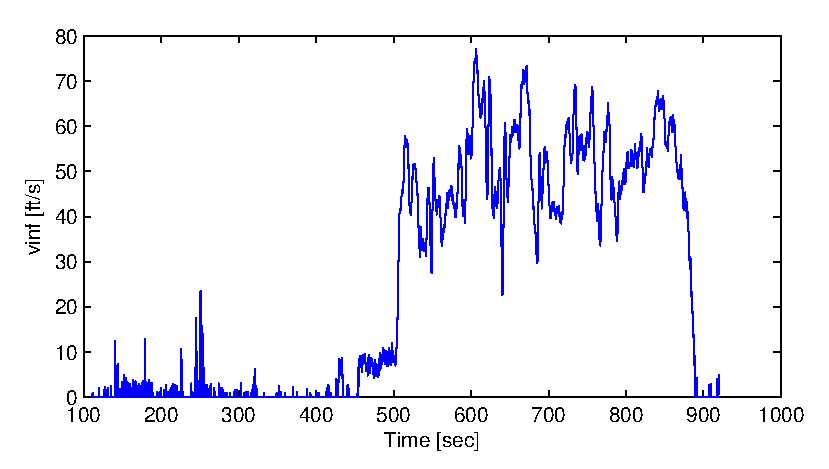
\includegraphics[width = 0.7\textwidth]{C:/Users/mufasa/Documents/Thesis/LaTex/figures/sampleOutput/State/vinf.eps}
\end{figure}
\begin{figure}[H]
	\centering
	\caption{alphaP vs. Time}
		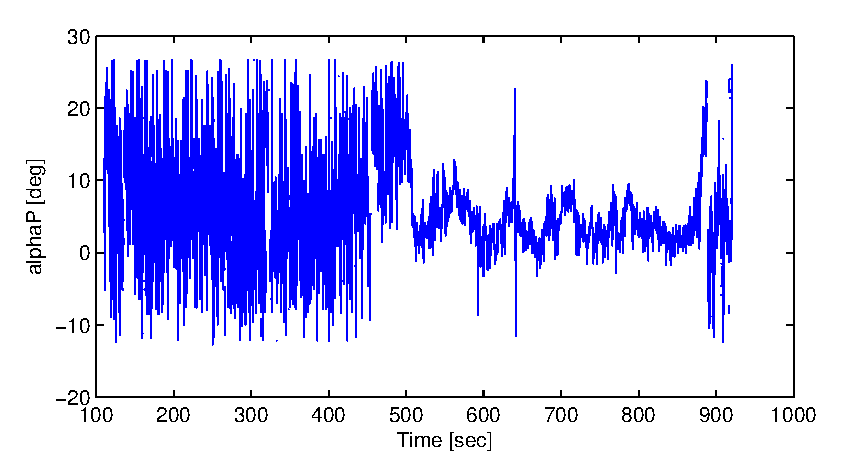
\includegraphics[width = 0.7\textwidth]{C:/Users/mufasa/Documents/Thesis/LaTex/figures/sampleOutput/State/alphaP.eps}
\end{figure}
\begin{figure}[H]
	\centering
	\caption{betaP vs. Time}
		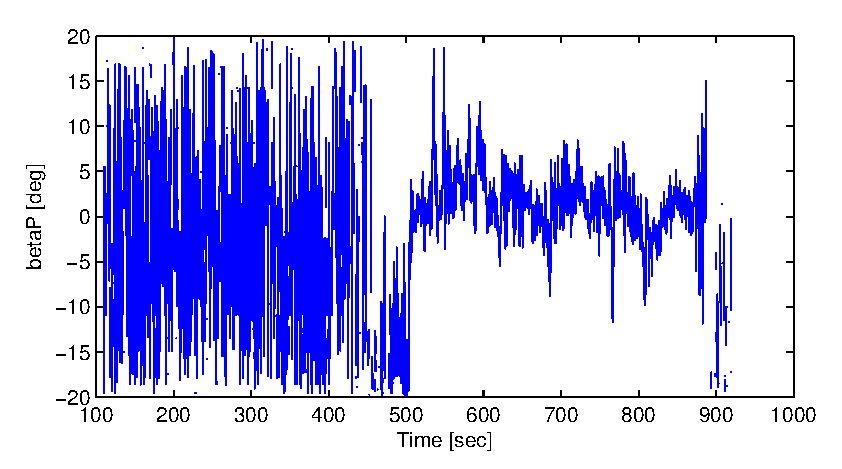
\includegraphics[width = 0.7\textwidth]{C:/Users/mufasa/Documents/Thesis/LaTex/figures/sampleOutput/State/betaP.eps}
\end{figure}
\begin{figure}[H]
	\centering
	\caption{rollRate vs. Time}
		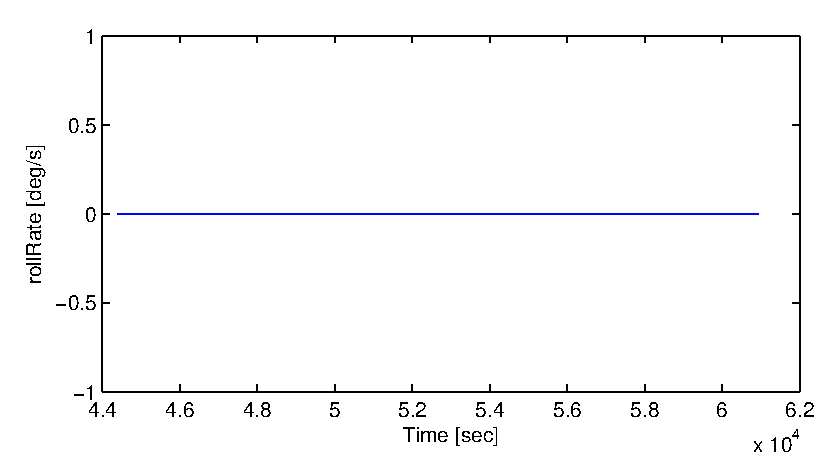
\includegraphics[width = 0.7\textwidth]{C:/Users/mufasa/Documents/Thesis/LaTex/figures/sampleOutput/State/rollRate.eps}
\end{figure}
\begin{figure}[H]
	\centering
	\caption{pitchRate vs. Time}
		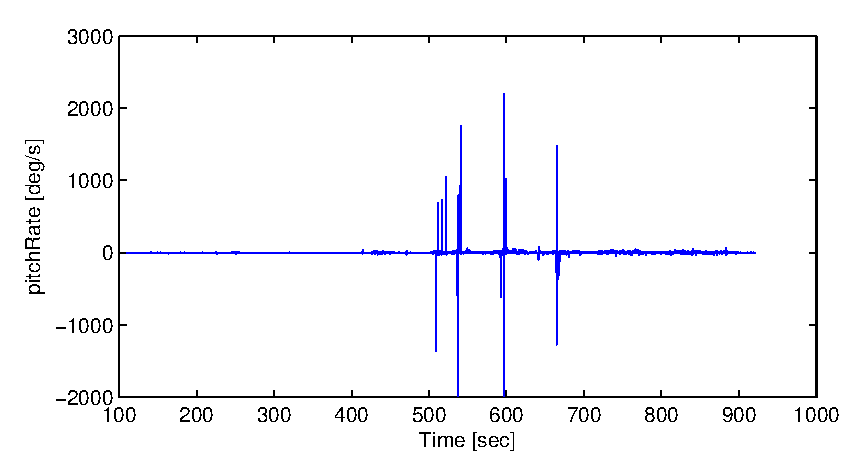
\includegraphics[width = 0.7\textwidth]{C:/Users/mufasa/Documents/Thesis/LaTex/figures/sampleOutput/State/pitchRate.eps}
\end{figure}
\begin{figure}[H]
	\centering
	\caption{yawRate vs. Time}
		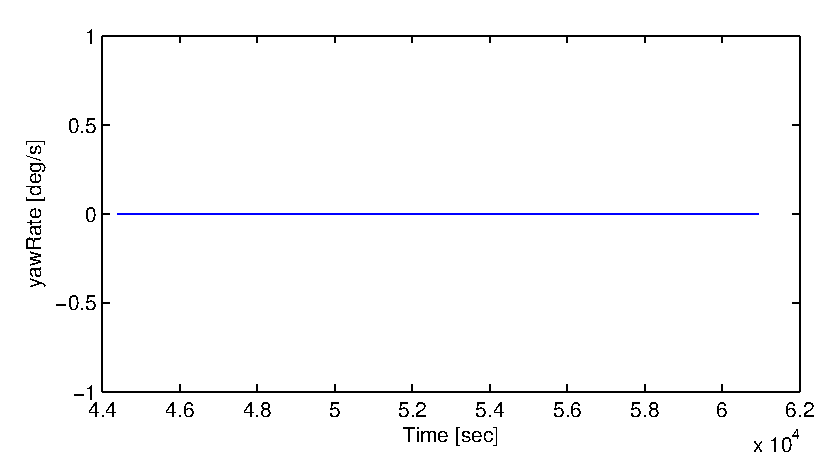
\includegraphics[width = 0.7\textwidth]{C:/Users/mufasa/Documents/Thesis/LaTex/figures/sampleOutput/State/yawRate.eps}
\end{figure}
\begin{figure}[H]
	\centering
	\caption{accelX vs. Time}
		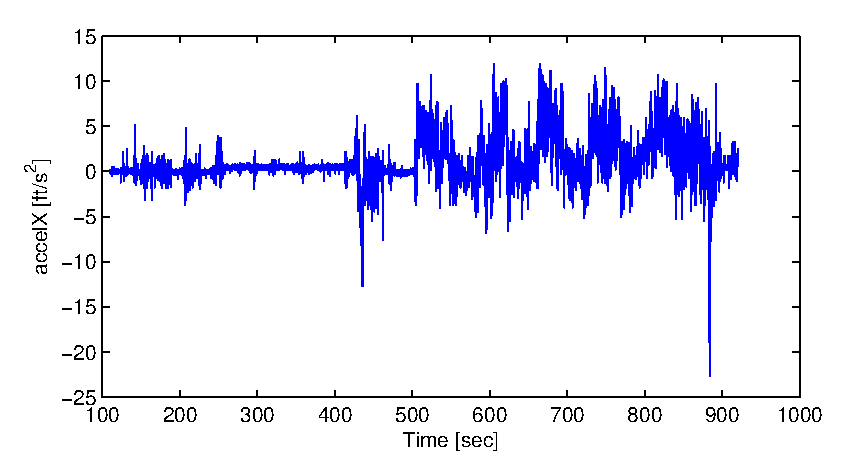
\includegraphics[width = 0.7\textwidth]{C:/Users/mufasa/Documents/Thesis/LaTex/figures/sampleOutput/State/accelX.eps}
\end{figure}
\begin{figure}[H]
	\centering
	\caption{accelY vs. Time}
		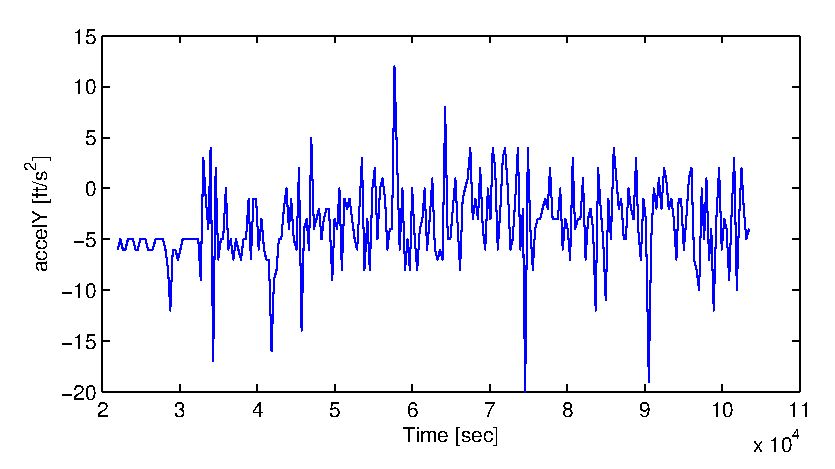
\includegraphics[width = 0.7\textwidth]{C:/Users/mufasa/Documents/Thesis/LaTex/figures/sampleOutput/State/accelY.eps}
\end{figure}
\begin{figure}[H]
	\centering
	\caption{accelZ vs. Time}
		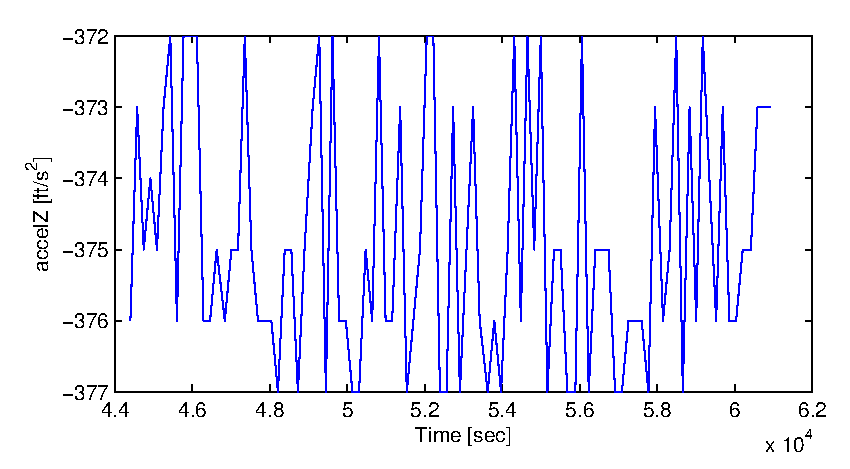
\includegraphics[width = 0.7\textwidth]{C:/Users/mufasa/Documents/Thesis/LaTex/figures/sampleOutput/State/accelZ.eps}
\end{figure}
\begin{figure}[H]
	\centering
	\caption{CD vs. Time}
		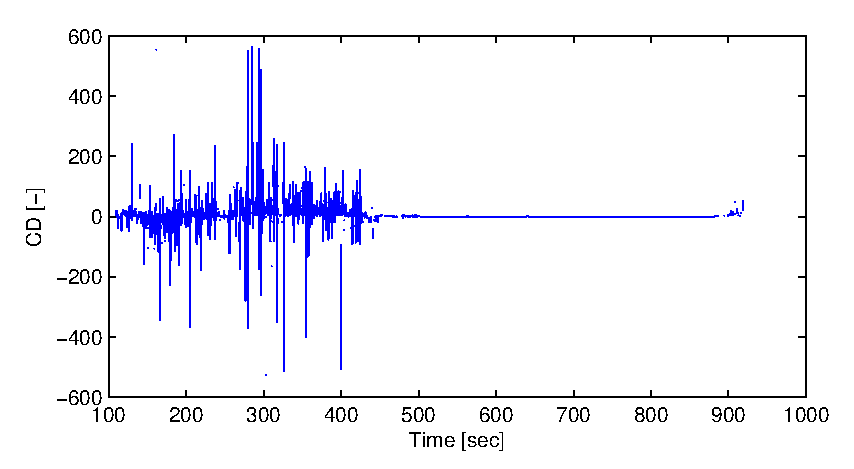
\includegraphics[width = 0.7\textwidth]{C:/Users/mufasa/Documents/Thesis/LaTex/figures/sampleOutput/State/CD.eps}
\end{figure}
\begin{figure}[H]
	\centering
	\caption{CY vs. Time}
		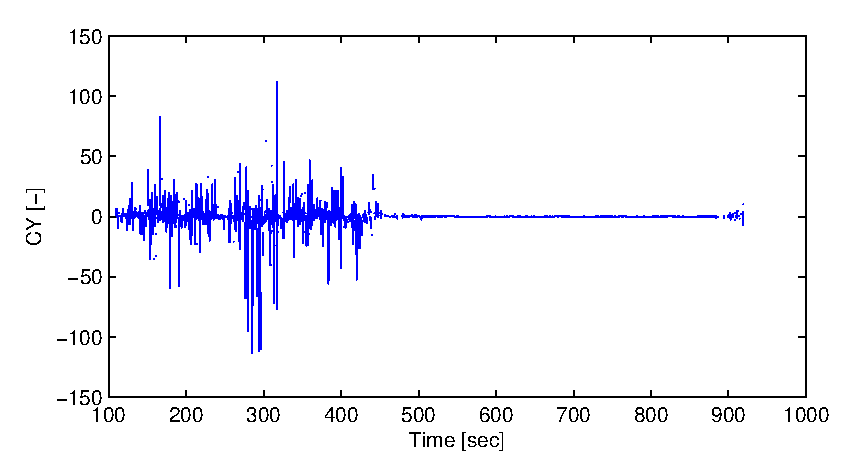
\includegraphics[width = 0.7\textwidth]{C:/Users/mufasa/Documents/Thesis/LaTex/figures/sampleOutput/State/CY.eps}
\end{figure}
\begin{figure}[H]
	\centering
	\caption{CL vs. Time}
		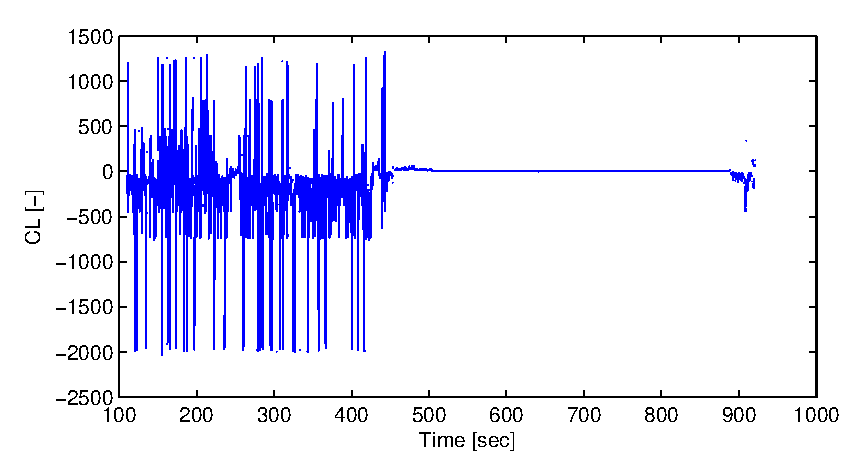
\includegraphics[width = 0.7\textwidth]{C:/Users/mufasa/Documents/Thesis/LaTex/figures/sampleOutput/State/CL.eps}
\end{figure}
\begin{figure}[H]
	\centering
	\caption{D vs. Time}
		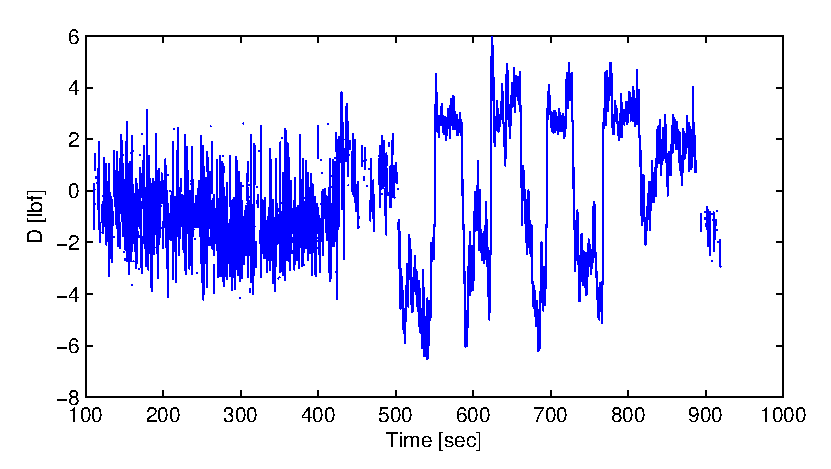
\includegraphics[width = 0.7\textwidth]{C:/Users/mufasa/Documents/Thesis/LaTex/figures/sampleOutput/State/D.eps}
\end{figure}
\begin{figure}[H]
	\centering
	\caption{Y vs. Time}
		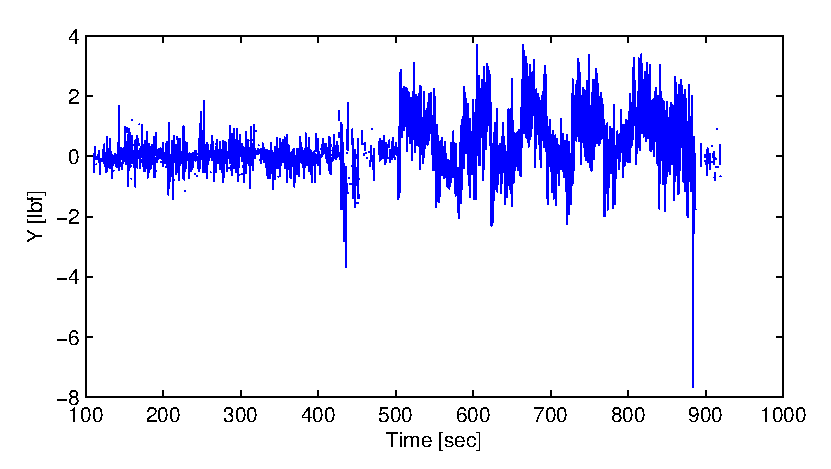
\includegraphics[width = 0.7\textwidth]{C:/Users/mufasa/Documents/Thesis/LaTex/figures/sampleOutput/State/Y.eps}
\end{figure}
\begin{figure}[H]
	\centering
	\caption{L vs. Time}
		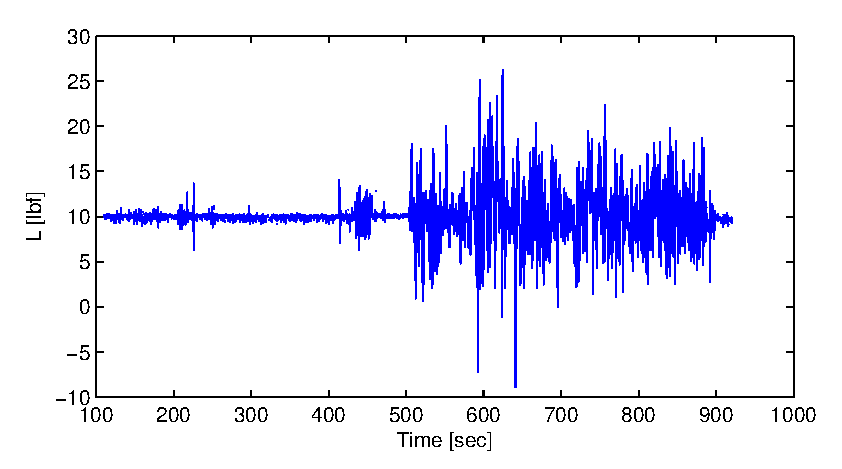
\includegraphics[width = 0.7\textwidth]{C:/Users/mufasa/Documents/Thesis/LaTex/figures/sampleOutput/State/L.eps}
\end{figure}
